\documentclass[11pt, oneside]{article} 
\usepackage{geometry}
\geometry{letterpaper} 
\usepackage{graphicx}
	
\usepackage{amssymb}
\usepackage{amsmath}
\usepackage{parskip}
\usepackage{color}
\usepackage{hyperref}

\graphicspath{{/Users/telliott/Github/precalculus/fig/}}
% \begin{center} \includegraphics [scale=0.4] {gauss3.png} \end{center}

\title{Ceva's theorem}
\date{}

\begin{document}
\maketitle
\Large

There are some special points in triangles including orthocenters, which we've already mentioned, but also circumcenters, incenters and centroids.

They have the common feature that three lines are drawn crossing at a single point.  We need to establish the conditions under which this assertion is true.

We begin with the triangle shown below, picking a point $P$ to be \emph{any point} inside the triangle.  Now draw line segments from each vertex through $P$ and extend them to the opposing side.
\begin{center} 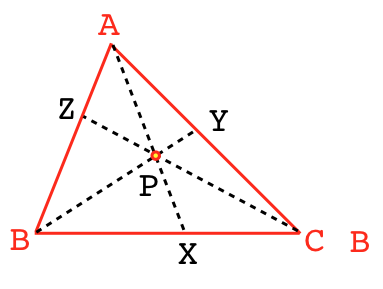
\includegraphics [scale=0.4] {Ceva1.png} \end{center}
Since $P$ can be anywhere, the ratio can be anything. Let's call it $x$.

\[ \frac{BX}{XC} = x \]

Line $AX$ divides the whole triangle into two parts.  

\begin{center} 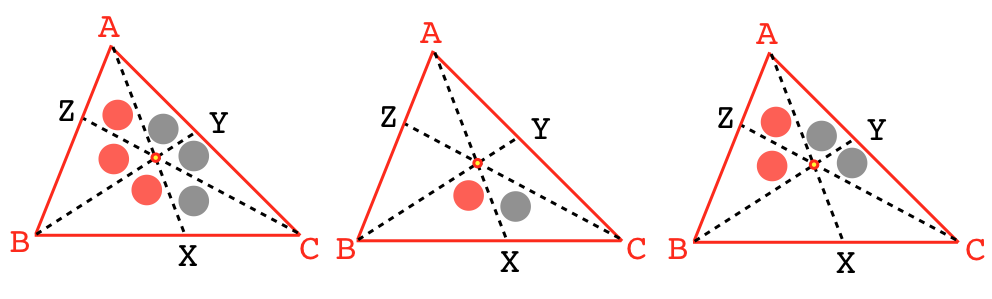
\includegraphics [scale=0.4] {Ceva2.png} \end{center}

We know that the area of $\triangle ABX$ is in the same proportion to the area of $\triangle AXC$ as $x$, because they share the same height, while $x$ is the ratio of their bases.  

\[ BX = x \cdot XC \]
\[ A_{ABX} = \frac{1}{2} h \cdot BX = \frac{1}{2} hx \cdot XC = x A_{AXC} \]

Now consider the lower pair of triangles $\triangle BPX$ and $\triangle CPX$

These two also have their areas in the ratio $x$, for the same reason.
\begin{center} 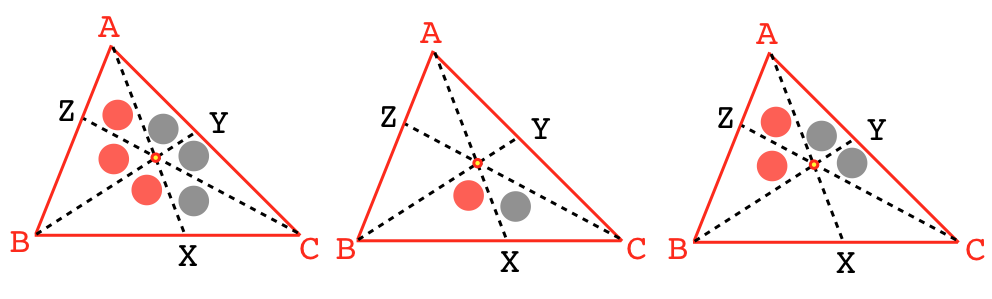
\includegraphics [scale=0.4] {Ceva2.png} \end{center}

By subtraction, $\triangle ABP$ and $\triangle ACP$ also have ratio $x$.

So, altogether, we have that
\[ \frac{BX}{XC} = \frac{|ABX|}{|ACX|} = \frac{|BPX|}{|CPX|} = \frac{|ABP|}{|ACP|} = x \]

\subsection*{more sides}

By the same reasoning, if $y=CY/YA$
\[ \frac{|BCP|}{|ABP|} = y \]
\begin{center} 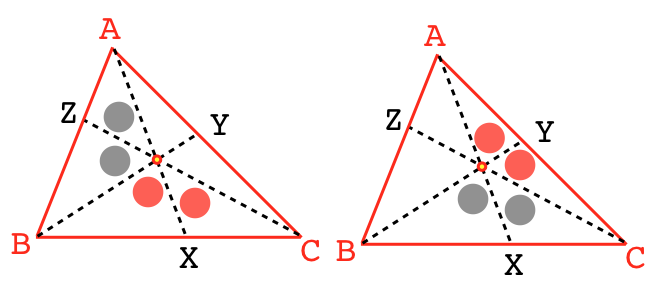
\includegraphics [scale=0.4] {Ceva3.png} \end{center}

and if $z= AZ/ZB$
\[ \frac{|ACP|}{|BCP|} = z \]

Then
\[ xyz = \frac{|ABP|}{|ACP|} \ \frac{|BCP|}{|ABP|} \ \frac{|ACP|}{|BCP|} \]

But all terms cancel, so
\[ xyz = 1 \]
And this is of course true not just for the areas but for the original line segments
\[ xyz = \frac{BX}{XC} \ \frac{CY}{YA} \ \frac{AZ}{ZB} = 1 \]

$\square$

This proof also works in reverse,
\[ xyz = 1 \iff \text{3 lines cross at point P} \]

We will just assume that part.

\subsection*{orthocenter}

So now, for this triangle
\begin{center} 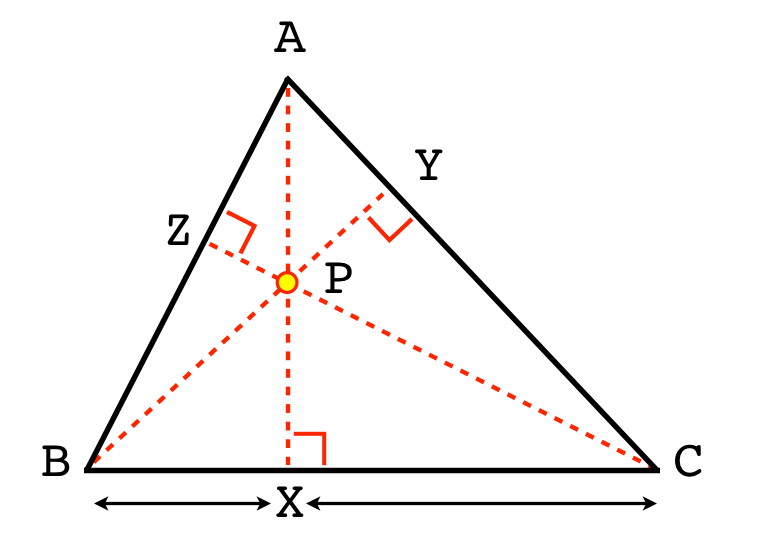
\includegraphics [scale=0.25] {ceva4.png} \end{center}

if $\alpha$ is the angle at vertex $A$ and so on, then for example,
\[ BX = AB \ cos \beta \]

and 
\[ \frac{BX}{XC} = \frac{AB \ cos \beta}{AC \ cos \gamma} \]
\[ \frac{CY}{YA} = \frac{BC \ cos \gamma}{AB \ cos \alpha} \]
\[ \frac{AZ}{ZB} = \frac{AC \ cos \alpha}{BC \ cos \beta} \]

When we construct this ratio, all the terms cancel.
\[ \frac{AB cos \beta}{AC \ cos \gamma} \ 
\frac{BC \ cos \gamma}{AB \ cos \alpha} \ 
\frac{AC \ cos \alpha}{BC \ cos \beta} = 1 \]

which means that 
\[ \frac{BX}{XC} \ \frac{CY}{YA} \ \frac{AZ}{ZB} = 1 \]

Therefore, the 3 altitudes all cross at a single point.  That point is the orthocenter, and this is a proof that it exists.

$\square$


\end{document}